\chapter{OCL Interpretation}
\label{chapter:interpretation}

\begin{flushright}
\textit{Chapter written by Claas Wilke}
\end{flushright}

This chapter describes how the \acs{OCL} Interpreter provided with DresdenOCL 
can be used. How to install and run \keyword{Dresden OCL2 for Eclipse} and how 
to load models and OCL constraints was explained in 
Chapter~\ref{chapter:introduction}. If you are not familiar with such basic uses
of DresdenOCL, read Chapter~\ref{chapter:introduction} first.



\section{The Simple Example}

This Chapter uses the \keyword{Simple Example} which is provided with 
\acl{DOT4Eclipse} located in the plug-in 
\reference{tudresden.ocl20.pivot.examples.\linebreak[0]simple}. An overview over
all examples provided with \acl{DOT4Eclipse} can be found in 
Table~\ref{tab:examples} in the appendix of this manual. An introduction into
the Simple Example can be found in Section~\ref{intro:simpleExample}. The model 
of the example defines three classes: The class \model{Person} has the 
attributes \model{age} and \model{name}. Two subclasses of \model{Person} are 
defined, \model{Student} and \model{Professor}.

To import the Simple Example into our Eclipse workspace we create a new Java 
project called \model{tudresden.ocl20.pivot.examples.\linebreak[0]simple} and 
use the import wizard \eclipse{General > Archive File} to import the example 
provided as a jar archive. In the following window we select the directory where
the jar file is located (probably the \model{plugins} directory into the Eclipse
root folder), select the archive 
\model{tudresden.ocl20.pivot.examples.simple.\linebreak[0]jar} and push the 
\eclipse{Finish} button (if you use a source code distribution of 
\acl{DOT4Eclipse} instead, you can simply import the project 
\model{tudresden.ocl20.\linebreak[0]pivot.examples.simple} using the import 
wizard \eclipse{General -> Existing Projects into Workspace}). 
Figure~\ref{pic:example:simple02} shows the \eclipse{Package Explorer}
containing the imported project.

\begin{figure}[!p]
	\centering
	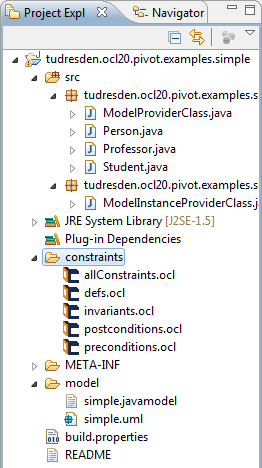
\includegraphics[width=0.5\linewidth]{figures/examples/simple02}
	\caption{The Package Explorer containing the Project which is required to run this Tutorial.}
	\label{pic:example:simple02}
	
	\vspace{4.0em}

  \lstset{
    language=OCL
  }
  \begin{lstlisting}[caption={The Constraints contained in the Constraint File.}, captionpos=b, label=lst:interpret:allConstraints]
-- The age of Person can not be negative.
context Person
inv: age >= 0

-- Students should be 16 or older.
context Student
inv: age > 16

-- Proffesors should be at least 30.
context Professor
inv: not (age < 30)

-- Returns the age of a Person.
context Person
def: getAge(): Integer = age

-- Before returning the age, the age must be defined.
context Person::getAge()
pre: not age.oclIsUndefined()

-- The result of getAge must equal to the age of a Person.
context Person::getAge()
post: result = age
  \end{lstlisting}
\end{figure}

The project provides a model file that contains a class diagram (the model file 
is located at \model{model/simple.uml}) and the constraint file we want to
interpret (located at 
\model{constraints\linebreak[0]/\linebreak[0]all\-Con\-straints.ocl}). 
Listing~\ref{lst:interpret:allConstraints} shows the constraints defined in the
constraint file.

First, the constraint file defines three simple invariants that ensure that 
the \model{age} of every \model{Person} must always zero or greater than zero. 
Furthermore, the \model{age} of every \model{Student} must be greater than
\model{16} and the \model{age} of every \model{Professor} does not have to be
lesser than \model{30}.

In addition to that the constraint file contains a definition constraint that 
defines a new operation \model{getAge()} which returns the \model{age} of a 
\model{Person}. A precondition checks, that the \model{age} must be defined 
before it can be returned by the operation \model{getAge()}. And finally, a 
postcondition which checks, whether or not the result of the operation 
\model{getAge()} is the same as the \model{age} of the \model{Person}.



\section{Preparation of the Interpretation}

To prepare the interpretation we have to import the model 
\model{model/simple.uml} for which we want to interpret constraints into the
\eclipse{Model Browser}. We use the model import wizard of DresdenOCL to import
the model. This procedure is explained in Section~\ref{intro:loadModel}. 
Furthermore, we have to import a model instance for which the constraints shall 
be interpreted into the \eclipse{Model Instance Browser}. We use another import 
wizard to import the model instance 
\model{bin/tudresden/ocl20/pivot/\linebreak[0]exam\-ples/\linebreak[0]simple\linebreak[0]/\linebreak[0]ModelProviderClass.class}.
Finally, we have to open the constraint file 
\model{con\-straints/\linebreak[0]all\-Con\-straints\linebreak[0].ocl}
containing the constraints we want to interpret. Afterwards, the \eclipse{Model
Browser} should look like illustrated in Figure~\ref{pic:interpret:prepare01} 
and the \eclipse{Model Instance Browser} should look like shown in 
Figure~\ref{pic:interpret:prepare02}.

\begin{figure}[!p]
	\centering
	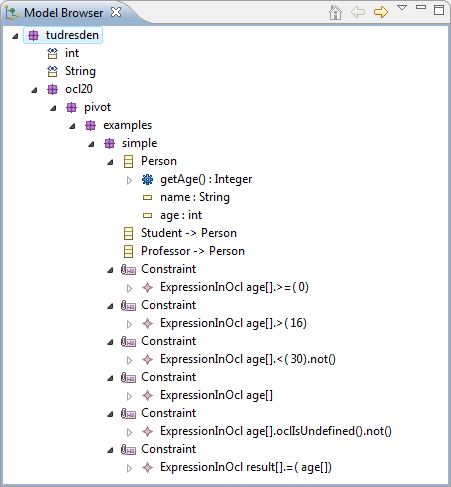
\includegraphics[width=0.6\linewidth]{figures/interpreter/prepare01}
	\caption{The Model Browser containing the Simple Model and its Constraints.}
	\label{pic:interpret:prepare01}

  \vspace{4.0em}
  
	\centering
	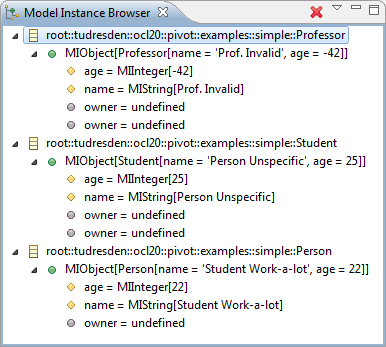
\includegraphics[width=0.6\linewidth]{figures/interpreter/prepare02}
	\caption{The Model Instance Browser containing the Simple Model Instance.}
	\label{pic:interpret:prepare02}
\end{figure}

The opened model instance contains three instances of the classes defined in the
Simple Example model. One instance of \model{Person}, one instance of 
\model{Student} and one instance of \model{Professor}. For these three instances
we now want to interpret the imported constraints.



\section{OCL Interpretation}

Now we can start the interpretation. To open the \acs{OCL} Interpreter we use 
the menu option \eclipse{Dresden OCL2 > Open OCL2 Interpreter}. The 
\eclipse{OCL Interpreter View} should now be visible (see 
Figure~\ref{pic:interpret:interpret01}).

By now, the \eclipse{OCL Interpreter View} does not contain any result. Besides
the results table, the view provides four buttons to control the \acs{OCL} 
Interpreter. The buttons are shown in Figure~\ref{pic:interpret:interpret02}. 
With the first button (from left to right) constraints can be prepared for 
interpretation. The second button can be used to add variables to the 
\keyword{Interpreter's Environment}. The third button provides the core 
functionality, it can be used to start the interpretation. And finally, the 
fourth button provides the possibility to delete all results from the 
\eclipse{OCL Interpreter View}. The functionality of the buttons will be 
explained below.

\begin{figure}[!p]
	\centering
	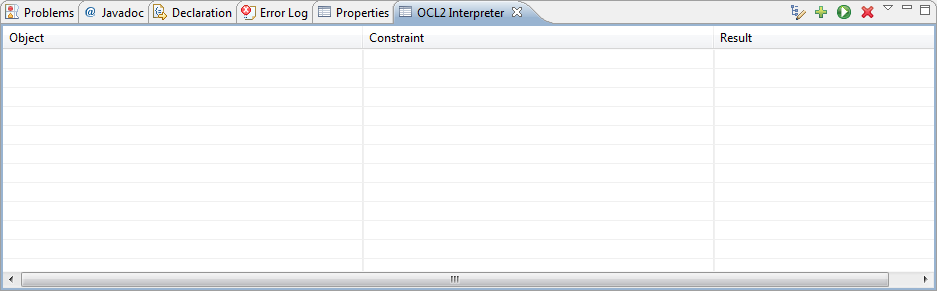
\includegraphics[width=1.0\linewidth]{figures/interpreter/interpret01}
	\caption{The OCL2 Interpreter View containing no results.}
	\label{pic:interpret:interpret01}

  \vspace{3.0em}
  
	\centering
	
\includegraphics[width=0.5\linewidth]{figures/interpreter/interpret02}
	\caption{The Buttons to Control the OCL2 Interpreter.}
	\label{pic:interpret:interpret02}

  \vspace{3.0em}

	\centering
	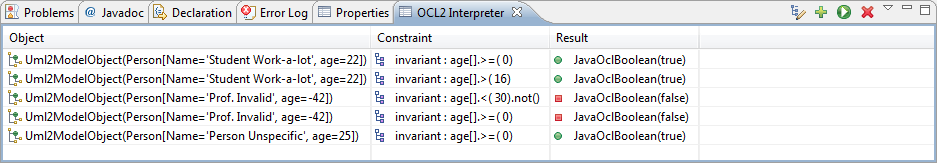
\includegraphics[width=1.0\linewidth]{figures/interpreter/interpret04}
	\caption{The results of the three Invariants for all Model Instance Elements.}
	\label{pic:interpret:interpret04}

  \vspace{3.0em}

	\centering
	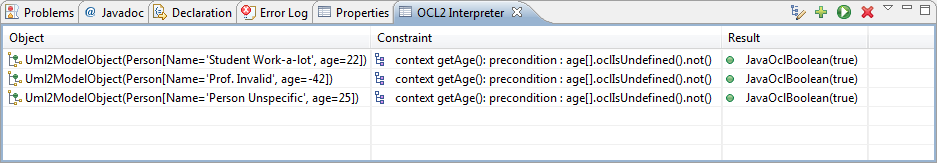
\includegraphics[width=1.0\linewidth]{figures/interpreter/interpret07}
	\caption{The results of the Definition for all Model Instance Elements.}
	\label{pic:interpret:interpret07}

\end{figure}


\subsection{Interpretation of Constraints}

To interpret constraints, we simple select them in the \eclipse{Model Browser} 
and push the button to interpret constraints (the third button from the left). 
First, we want to interpret the three invariants defining the range of the 
\model{age} of \model{Persons}, \model{Students} and \model{Professors}. We 
select them in the \eclipse{Model Browser} and push the \eclipse{Interpret} button.
The result of the interpretation is now shown in the \eclipse{\acs{OCL}
Interpreter View} (see Figure~\ref{pic:interpret:interpret04}).

The invariant \model{age >= 0} has been interpreted for all three model objects.
The results for the \model{Person} and the \model{Student} instances are 
\model{true} because their \model{age} is greater than zero. The result for the
\model{Professor} instance is \model{false} because its \model{age} is 
\model{-42}.

The two other invariants were only interpreted for the \model{Student} or the 
\model{Pro\-fessor} instance because their context is not the class 
\model{Person} but the class \model{Student} or the class \model{Professor}, 
respectively. Again, the \model{Student's} result is \model{true} and the 
\model{Professor's} result is \model{false}.

Besides invariants, \acs{OCL}~2.2 enables us to use \acs{OCL} expressions to
define new attributes and methods or to initialize attributes and methods. Such
\model{def}, \model{init} and \model{body} constraints cannot be interpreted to
\model{true} or \model{false}, because their result type has not to be 
\model{Boolean}. Furthermore, they can be used to alter the results of other 
constraints that shall be interpreted. The \model{allConstraints.ocl} file 
contains a definition constraint, which defines the method \model{getAge()} for 
the class \model{Person}. Now, we want to interpret this definition constraint. 
We select the constraint in the \eclipse{Model Browser} and push the \eclipse{Interpret} button.
The result of the interpretation is shown in 
Figure~\ref{pic:interpret:interpret07}. The interpretation finishes for all
three instances successfully because the attribute \model{age} has been set for 
all three instances.


\subsection{Adding Variables to the Environment}

When interpreting OCL constraints from the GUI, we have to add further context 
information to interpret some pre- and postconditions. For example, the 
postcondition contained in the constraint file compares the result of the 
method \model{getAge()} with the attribute \model{age} of the referenced 
\model{Person} instance. Therefore, \acs{OCL} provides the special variable 
\model{result} in postconditions which contains the result of the constrained 
method's execution. Using the \eclipse{\acs{OCL} Interpreter View} we cannot 
execute the method \model{getAge()} and store the result in the \model{result} 
variable. We can interpret the postcondition in a specific context which has to 
be prepared by hand only. We have to set the result variable manually.

If we interpret the postcondition constraint (the sixth and last constraint in 
the \eclipse{Model Browser}) without setting the \model{result} variable, the 
constraint results in a \model{undefined} result for all three model instances
(see Figure~\ref{pic:interpret:interpret08}).

To prepare the variable, we push the button to add new variables to the 
Interpreter Environment (the second button from the left) and a new window opens
which we can use to specify new variables. We enter the name \model{result}, 
select the variable type \model{Integer} and enter the value \model{25}. Then we
push the \eclipse{OK} button (see Figure~\ref{pic:interpret:interpret09}. The 
result variable has now been added to the Interpreter's Environment.

\begin{figure}[!p]
	\centering
	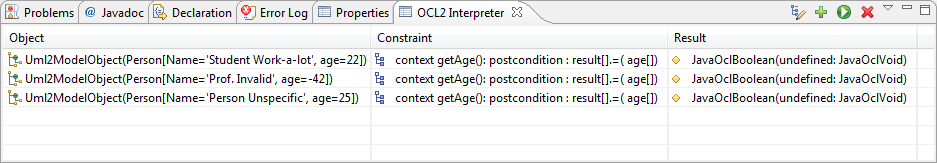
\includegraphics[width=1.0\linewidth]{figures/interpreter/interpret08}
	\caption{The results of the Postcondition without preparing the Result Variable.}
	\label{pic:interpret:interpret08}

  \vspace{3.0em}
	
	\centering
	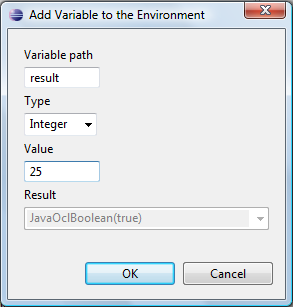
\includegraphics[width=0.5\linewidth]{figures/interpreter/interpret09}
	\caption{The Window to add new Variables to the Environment.}
	\label{pic:interpret:interpret09}

  \vspace{3.0em}
	
	\centering
	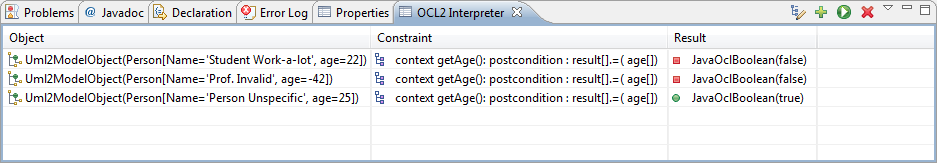
\includegraphics[width=1.0\linewidth]{figures/interpreter/interpret10}
	\caption{The Results of the Postcondition with Result Variable Preparation.}
	\label{pic:interpret:interpret10}
	
  \vspace{3.0em}

  \lstset{
    language=OCL
  }
  \begin{lstlisting}[caption={An example Precondition defined on an Operation with Argument.}, captionpos=b, label=lst:interpret:precondition]
-- arg01 must be defined.
context Person::setAge(arg01: Integer)
pre: not arg01.oclIsUndefined()
  \end{lstlisting}
\end{figure}

Now, we can interpret the postcondition again. The result is shown in 
Figure~\ref{pic:interpret:interpret10}. The results for the \model{Student} and
\model{Professor} instances are both \model{false} because their \model{age} 
attribute is not equal to \model{25} and thus the \model{result} value does not 
match to the \model{age} attribute. But the interpretation for the
\model{Person} instance succeeds because its \model{age} is \model{25}.

Other examples requiring manual addition of context information are pre- and
postconditions that are defined on operations containing arguments. 
Listing~\ref{lst:interpret:precondition} shows a precondition that is defined on
an operation \code{setAge(arg01)}. If the argument \code{arg01} is referred 
during interpretation, the interpreter has to know the value of the argument. 
Thus, we would have to add the value of \code{arg01} before the constraint's 
interpretation manually as shown for the \code{result} variable.


\subsection{Preparation of Constraints}

The interpretation of some postconditions requires a preparation of the 
Interpreter's environment before the operation defined in the context of the 
postcondition is invoked. Listing~\ref{lst:interpret:postcondition} shows such a
postcondition. The postcondition is defined on an operation 
\code{birthdayHappens()} that increments the \code{age} of a \code{Person}. The 
postcondition checks, whether the \code{age} was incremented or not. Thus, the 
Interpreter has to store the value of \code{age} before the operation 
\code{birthdayHappens()} is invoked. Therefore, the Interpreter View provides a 
button to prepare constraints (the first button from the left). If you want to 
interpret such postconditions, first select and prepare your constraint. The
value of \code{age@pre} is then stored in the Interpreter's environment. 
Then you can invoke your model instance's operation (which is quite 
complicate from the GUI). Afterwards you can interpret the postcondition.

\begin{figure}[!t]
  \lstset{
    language=OCL
  }
  \begin{lstlisting}[caption={An example Postcondition that must be prepared.}, captionpos=b, label=lst:interpret:postcondition]
-- age must be incremented by one.
context Person::birthdayHappens()
post: age = age@pre + 1
  \end{lstlisting}
\end{figure}

The preparation of postconditions is not that useful when interpreting 
constraints from the GUI of DresdenOCL because you cannot invoke your 
operations here to alter your model instance's state. Nevertheless, like the 
possibility to add variables to the Interpreter's environment you can prepare 
postconditions from the GUI. These operations are much more useful when using 
DresdenOCL via its API and using the \acs{OCL} Interpreter to check \acs{OCL} 
constraints during the runtime of other software. Then you can prepare
constraints before methods are invoked and check postconditions afterwards, 
e.g., by using \emph{\acf{AOP}}.



\section{Summary}
  
This chapter described how \acs{OCL} constraints can be interpreted using the 
\acs{OCL} Interpreter of DresdenOCL. The preparation and interpretation of 
constraints has been explained, the addition of new variables to the 
Interpreter Environment has been shown. Besides the use of the Interpreter via 
DresdenOCL's GUI, you can also invoke the Interpreter via DresdenOCL's 
\acs{API}. The easiest way to connect to DresdenOCL is via its \emph{Facade} 
providing interfaces for all services of DresdenOCL. How to use DresdenOCL's 
facade is documented in Chapter~\ref{chapter:integration}.
